\chapter{Arrays and references}

%NOTE: DW liked the previous version where strings come before arrays
% CSM: the transition is better from strings to things to objects
% Plus we moved command-line arguments to the strings chapter

Up to this point, the only variables we have used were for individual values such as numbers or strings.
In this chapter, we'll learn how to store multiple values of the same type using a single variable.
This language feature will enable you to write programs that manipulate larger amounts of data.


\section{Creating arrays}

\index{array}
\index{element}

An {\bf array} is a sequence of values; the values in the array are called {\bf elements}.
You can make an array of \java{int}s, \java{double}s, or any other type, but all the values in an array must have the same type.

\index{type!array}

To create an array, you have to declare a variable with an {\em array type} and then create the array itself.
Array types look like other Java types, except they are followed by square brackets (\java{[]}).
For example, the following lines declare that \java{counts} is an ``integer array'' and \java{values} is a ``double array'':

\begin{code}
int[] counts;
double[] values;
\end{code}

\index{new}
\index{operator!new}

To create the array itself, you have to use the \java{new} operator, which we first saw in Section~\ref{scanner}:

\begin{code}
counts = new int[4];
values = new double[size];
\end{code}

The first assignment makes \java{count} refer to an array of four integers.
The second makes \java{values} refer to an array of \java{double}, where the number of elements in \java{values} depends on the value of \java{size}.

Of course, you can also declare the variable and create the array in a single line of code:

\begin{code}
int[] counts = new int[4];
double[] values = new double[size];
\end{code}

\index{NegativeArraySizeException}
\index{exception!NegativeArraySize}

You can use any integer expression for the size of an array, as long as the value is nonnegative.
If you try to create an array with $-4$ elements, for example, you will get a \java{NegativeArraySizeException}.
An array with zero elements is allowed, and there are special uses for such arrays that we'll see later on.


\section{Accessing elements}
\label{elements}

\index{memory diagram}
\index{diagram!memory}

When you create an array of \java{int}s, the elements are initialized to zero.
Figure~\ref{fig.array} shows a memory diagram of the \java{counts} array so far.

\begin{figure}[!ht]
\begin{center}
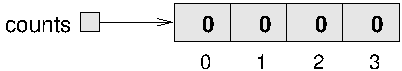
\includegraphics{figs/array.pdf}
\caption{Memory diagram of an \java{int} array.}
\label{fig.array}
\end{center}
\end{figure}

\index{reference}

The arrow indicates that the value of \java{counts} is a {\bf reference} to the array.
You should think of {\em the array} and {\em the variable} that refers to it as two different things.
As we'll soon see, we can assign a different variable to refer to the same array, and we can change the value of \java{counts} to refer to a different array.

\index{element}
\index{index}
\index{array!element}
\index{array!index}

The large numbers inside the boxes are the elements of the array.
The small numbers outside the boxes are the {\bf indexes} (or indices) used to identify each location in the array.
Notice that the index of the first element is 0, not 1, as you might have expected.

The \java{[]} operator selects elements from an array:

\begin{code}
System.out.println("The zeroth element is " + counts[0]);
\end{code}

You can use the \java{[]} operator anywhere in an expression:

\begin{code}
counts[0] = 7;
counts[1] = counts[0] * 2;
counts[2]++;
counts[3] -= 60;
\end{code}

Figure~\ref{fig.array2} shows the result of these statements.

\begin{figure}[!ht]
\begin{center}
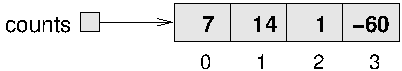
\includegraphics{figs/array2.pdf}
\caption{Memory diagram after several assignment statements.}
\label{fig.array2}
\end{center}
\end{figure}

You can use any expression as an index, as long as it has type \java{int}.
One of the most common ways to index an array is with a loop variable.
For example:

\begin{code}
int i = 0;
while (i < 4) {
    System.out.println(counts[i]);
    i++;
}
\end{code}

This \java{while} loop counts from 0 up to 4.
When \java{i} is 4, the condition fails and the loop terminates.
So the body of the loop is only executed when \java{i} is 0, 1, 2, and 3.

\index{loop variable}
\index{variable!loop}

Each time through the loop we use \java{i} as an index into the array, displaying the \java{i}th element.
This type of array processing is often written using a \java{for} loop.

\begin{code}
for (int i = 0; i < 4; i++) {
    System.out.println(counts[i]);
}
\end{code}

\index{ArrayIndexOutOfBoundsException}
\index{exception!ArrayIndexOutOfBounds}

For the \java{counts} array, the only legal indexes are 0, 1, 2, and 3.
If the index is negative or greater than 3, the result is an \java{ArrayIndexOutOfBoundsException}.


\section{Displaying arrays}
\label{printarray}

You can use \java{println} to display an array, but it probably doesn't do what you would like.
For example, the following fragment (1) declares an array variable, (2) makes it refer to an array of four elements, and (3) attempts to display the contents of the array using \java{println}:

\begin{code}
int[] a = {1, 2, 3, 4};
System.out.println(a);
\end{code}

Unfortunately, the output is something like:

\begin{stdout}
[I@bf3f7e0
\end{stdout}

The bracket indicates that the value is an array, \java{I} stands for ``integer'', and the rest represents the address of the array.
If we want to display the elements of the array, we can do it ourselves:

\begin{code}
public static void printArray(int[] a) {
    System.out.print("{" + a[0]);
    for (int i = 1; i < a.length; i++) {
        System.out.print(", " + a[i]);
    }
    System.out.println("}");
}
\end{code}

Given the previous array, the output of this method is:

\begin{stdout}
{1, 2, 3, 4}
\end{stdout}

\index{utility class}
\index{Arrays class}

The Java library provides a utility class \java{java.util.Arrays} that provides methods for working with arrays.
One of them, \java{toString}, returns a string representation of an array.
We can invoke it like this:

\begin{code}
System.out.println(Arrays.toString(a));
\end{code}

And the output is:

\begin{stdout}
[1, 2, 3, 4]
\end{stdout}

As usual, we have to import \java{java.util.Arrays} before we can use it.
Notice that the string format is slightly different: it uses square brackets instead of curly braces.
But it beats having to write the \java{printArray} method.


\section{Copying arrays}

\index{array!copying}

As explained in Section~\ref{elements}, array variables contain {\em references} to arrays.
When you make an assignment to an array variable, it simply copies the reference.
But it doesn't copy the array itself!
For example:

\begin{code}
double[] a = new double[3];
double[] b = a;
\end{code}

These statements create an array of three \java{double}s and make two different variables refer to it, as shown in Figure~\ref{fig.array3}.

\begin{figure}[!ht]
\begin{center}
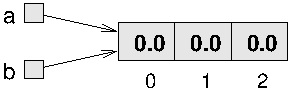
\includegraphics{figs/array3.pdf}
\caption{Memory diagram showing two variables that refer to the same array.}
\label{fig.array3}
\end{center}
\end{figure}

\index{alias}

Any changes made through either variable will be seen by the other.
For example, if we set \java{a[0] = 17.0}, and then display \java{b[0]}, the result is {\tt 17.0}.
Because \java{a} and \java{b} are different names for the same thing, they are sometimes called {\bf aliases}.

If you actually want to copy the array, not just a reference, you have to create a new array and copy the elements from the old to the new, like this:

\begin{code}
double[] b = new double[3];
for (int i = 0; i < 3; i++) {
    b[i] = a[i];
}
\end{code}

\index{Arrays class}

Another option is to use \java{java.util.Arrays}, which provides a method named \java{copyOf} that copies an array.
You can invoke it like this:

\begin{code}
double[] b = Arrays.copyOf(a, 3);
\end{code}

The second parameter is the number of elements you want to copy, so you can also use \java{copyOf} to copy just part of an array.


\section{Array length}

\index{length!array}
\index{array!length}

The examples in the previous section only work if the array has three elements.
It would be better to generalize the code to work with arrays of any size.
We can do that by replacing the magic number, \java{3}, with \java{a.length}:

\begin{code}
double[] b = new double[a.length];
for (int i = 0; i < a.length; i++) {
    b[i] = a[i];
}
\end{code}

All arrays have a built-in constant, \java{length}, that stores the number of elements.
The expression \java{a.length} may look like a method invocation, but there are no parentheses and no arguments.
%\java{length} is actually an {\bf attribute} of the array, not a method.
%We will learn more about attributes in Section~\ref{attribute}.

The last time this loop gets executed, \java{i} is \java{a.length - 1}, which is the index of the last element.
When \java{i} is equal to \java{a.length}, the condition fails and the body is not executed -- which is a good thing, because trying to access \java{a[a.length]} would throw an exception.

You can also use \java{a.length} with \java{Arrays.copyOf}:

\begin{code}
double[] b = Arrays.copyOf(a, a.length);
\end{code}


\section{Array traversal}
\label{traversal}

Many computations can be implemented by looping through the elements of an array and performing an operation on each element.
For example, the following loop squares the elements of a \java{double} array:

\begin{code}
for (int i = 0; i < a.length; i++) {
    a[i] = Math.pow(a[i], 2.0);
}
\end{code}

\index{traversal}
\index{search}

Looping through the elements of an array is called a {\bf traversal}.
Another common pattern is a {\bf search}, which involves traversing an array looking for a particular element.
For example, the following method takes an \java{int} array and an integer value, and it returns the index where the value appears:

\begin{code}
public static int search(double[] a, double target) {
    for (int i = 0; i < a.length; i++) {
        if (a[i] == target) {
            return i;
        }
    }
    return -1;
}
\end{code}

If we find the target value in the array, we return its index immediately.
If the loop exits without finding the target, it returns \java{-1}, a special value chosen to indicate a failed search.

\index{reduce}

Another common traversal is a {\bf reduce} operation, which ``reduces'' an array of values down to a single value.
Examples include the sum or product of the elements, the minimum, and the maximum.
The following method takes a \java{double} array and returns the sum of the elements:

\begin{code}
public static double sum(double[] a) {
    double total = 0.0;
    for (int i = 0; i < a.length; i++) {
        total += a[i];
    }
    return total;
}
\end{code}

\index{accumulator}

Before the loop, we initialize \java{total} to zero.
Each time through the loop, we update \java{total} by adding one element from the array.
At the end of the loop, \java{total} contains the sum of the elements.
A variable used this way is sometimes called an {\bf accumulator}.


\section{Random numbers}
\label{random}

\index{deterministic}

Most computer programs do the same thing every time they run; programs like that are {\bf deterministic}.
Usually determinism is a good thing, since we expect the same calculation to yield the same result.
But for some applications, we want the computer to be unpredictable.
Games are an obvious example, but there are many others.

%Technically speaking, all computer programs are deterministic: they simply execute the source code.

\index{nondeterministic}
\index{pseudorandom}

Making a program {\bf nondeterministic} turns out to be hard, because it's hard for a computer to generate truly random numbers.
But there are algorithms that generate unpredictable sequences called {\bf pseudorandom} numbers.
For most applications, they are as good as random.

%Nondeterminism is a theoretical concept for analyzing the complexity of algorithms.

\index{Random}
\index{nextInt!Random}

If you did Exercise~\ref{guess}, you have already seen \java{java.util.Random}, which generates pseudorandom numbers.
The method \java{nextInt} takes an integer argument, \java{n}, and returns a random integer between \java{0} and \java{n - 1} (inclusive).

If you generate a long series of random numbers, every value should appear, at least approximately, the same number of times.
One way to test this behavior of \java{nextInt} is to generate a large number of values, store them in an array, and count the number of times each value occurs.

The following method creates an \java{int} array and fills it with random numbers between 0 and 99.
The argument specifies the size of the array, and the return value is a reference to the new array.

\begin{code}
public static int[] randomArray(int size) {
    Random random = new Random();
    int[] a = new int[size];
    for (int i = 0; i < a.length; i++) {
        a[i] = random.nextInt(100);
    }
    return a;
}
\end{code}

The following fragment generates an array and displays it using \java{printArray} from Section~\ref{printarray}:

\begin{code}
int numValues = 8;
int[] array = randomArray(numValues);
printArray(array);
\end{code}

The output looks like this:

\begin{stdout}
{15, 62, 46, 74, 67, 52, 51, 10}
\end{stdout}

If you run it, you will probably get different values.


\section{Traverse and count}

\index{histogram}
\index{counter}

If these values were exam scores -- and they would be pretty bad exam scores -- the teacher might present them to the class in the form of a {\bf histogram}.
In statistics, a histogram is a set of counters that keeps track of the number of times each value appears.

For exam scores, we might have ten counters to keep track of how many students scored in the 90s, the 80s, etc.
To do that, we can traverse the array and count the number of elements that fall in a given range.

The following method takes an array and two integers, \java{low} and \java{high}.
It returns the number of elements that fall in the range from  \java{low} to \java{high}.

\begin{code}
public static int inRange(int[] a, int low, int high) {
    int count = 0;
    for (int i = 0; i < a.length; i++) {
        if (a[i] >= low && a[i] < high) {
            count++;
        }
    }
    return count;
}
\end{code}

\index{reduce}

This pattern should look familiar: it is another reduce operation.
Notice that \java{low} is included in the range (\java{>=}), but \java{high} is excluded (\java{<}).
This detail keeps us from counting any scores twice.

Now we can count the number of scores in each grade range:

\begin{code}
int[] scores = randomArray(30);
int a = inRange(scores, 90, 100);
int b = inRange(scores, 80, 90);
int c = inRange(scores, 70, 80);
int d = inRange(scores, 60, 70);
int f = inRange(scores, 0, 60);
\end{code}


\section{Building a histogram}

The previous code is repetitious, but it is acceptable as long as the number of ranges is small.
But suppose we wanted to keep track of the number of times each score appears.
We would have to write 100 lines of code:

\begin{code}
int count0 = inRange(scores, 0, 1);
int count1 = inRange(scores, 1, 2);
int count2 = inRange(scores, 2, 3);
...
int count99 = inRange(scores, 99, 100);
\end{code}

What we need is a way to store 100 counters, preferably so we can use an index to access them.
In other words, we need another array!

The following fragment creates an array of 100 counters, one for each possible score.
It loops through the scores and uses \java{inRange} to count how many times each score appears.
Then it stores the results in the array:

\begin{code}
int[] counts = new int[100];
for (int i = 0; i < counts.length; i++) {
    counts[i] = inRange(scores, i, i + 1);
}
\end{code}

Notice that we are using the loop variable \java{i} three times: as an index into the \java{counts} array, and as two arguments for \java{inRange}.

The code works, but it is not as efficient as it could be.
Every time the loop invokes \java{inRange}, it traverses the entire array.

\index{efficiency}

It would be better to make a single pass through the array, and for each score, compute which range it falls in and increment the corresponding counter.
This code traverses the array of scores {\em only once} to generate the histogram:

\begin{code}
int[] counts = new int[100];
for (int i = 0; i < scores.length; i++) {
    int index = scores[i];
    counts[index]++;
}
\end{code}

Each time through the loop, it selects one element from \java{scores} and uses it as an index to increment the corresponding element of \java{counts}.
Because this code only traverses the array of scores once, it is much more efficient.


\section{The enhanced for loop}
\label{enhanced}

Since traversing arrays is so common, Java provides an alternative syntax that makes the code more compact.
For example, consider a \java{for} loop that displays the elements of an array on separate lines:

\begin{code}
for (int i = 0; i < values.length; i++) {
    int value = values[i];
    System.out.println(value);
}
\end{code}

We could rewrite the loop like this:

\begin{code}
for (int value : values) {
    System.out.println(value);
}
\end{code}

\index{enhanced for loop}

This statement is called an {\bf enhanced for loop}.
You can read it as, ``for each \java{value} in \java{values}''.
It's conventional to use plural nouns for array variables and singular nouns for element variables.

Notice how the single line \java{for (int value : values)} replaces the first two lines of the standard \java{for} loop.
It hides the details of iterating each index of the array, and instead, focuses on the values themselves.

Using the enhanced \java{for} loop, and removing the temporary variable, we can write the histogram code from the previous section more concisely:

\begin{code}
int[] counts = new int[100];
for (int score : scores) {
    counts[score]++;
}
\end{code}

Enhanced \java{for} loops often make the code more readable, especially for accumulating values.
But they are not helpful when you need to refer to the index, as in search operations.

\begin{code}
for (double d : array) {
    if (d == target) {
        // array contains d, but we don't know the index
    }
}
\end{code}

\index{toCharArray}

Unfortunately, the enhanced \java{for} loop does not work with strings.
But you can convert any string to a character array and iterate that:

\begin{code}
for (char letter : fruit.toCharArray()) {
    System.out.println(letter);
}
\end{code}

%TODO put this somewhere
Do not confuse \java{string.length()}, which is a method, with \java{array.length}, which is a constant.


\section{Vocabulary}

\begin{description}

\term{array}
A collection of values, where all the values have the same type, and each value is identified by an index.

\term{element}
One of the values in an array.
The \java{[]} operator selects elements.

%\term{index}
%An integer variable or value used to indicate an element of an array.

\term{reference}
A value that indicates another value, like an array.
In a memory diagram, a reference appears as an arrow.

\term{alias}
A variable that refers to the same object as another variable.

\term{traversal}
Looping through the elements of an array (or other collection).

\term{search}
A traversal pattern used to find a particular element of an array.

\term{reduce}
A traversal pattern that combines the elements of an array into a single value.

\term{accumulator}
A variable used to accumulate results during a traversal.

\term{deterministic}
A program that does the same thing every time it is invoked.

\term{nondeterministic}
A program that always behaves differently, even when run multiple times with the same input.

\term{pseudorandom}
A sequence of numbers that appear to be random, but which are actually the product of a deterministic computation.

\term{histogram}
An array of integers where each integer counts the number of values that fall into a certain range.

\term{enhanced for loop}
An alternative syntax for traversing the elements (values) of an array.

\end{description}


\section{Exercises}

The code for this chapter is in the {\tt ch07} directory of {\tt ThinkJavaCode2}.
See page~\pageref{code} for instructions on how to download the repository.
Before you start the exercises, we recommend that you compile and run the examples.

If you haven't already, take a look at Appendix~\ref{debugging} where we've collected some of our favorite debugging advice.
It refers to language features we haven't yet covered, but it's good for you to know what's available when you need it.


\begin{exercise}  %%V6 Ex8.1

The goal of this exercise is to practice encapsulation with some of the examples in this chapter.

\begin{enumerate}

\item Starting with the code in Section~\ref{traversal}, write a method called \java{powArray} that takes a \java{double} array, \java{a}, and returns a new array that contains the elements of \java{a} squared.
Generalize it to take a second argument and raise the elements of \java{a} to the given power.

\item Starting with the code in Section~\ref{enhanced}, write a method called \java{histogram} that takes an \java{int} array of scores from 0 to (but not including) 100, and returns a histogram of 100 counters.
Generalize it to take the number of counters as an argument.

\end{enumerate}

\end{exercise}


\begin{exercise}  %%V6 Ex8.2

The purpose of this exercise is to practice reading code and recognizing the traversal patterns in this chapter.
The following methods are hard to read, because instead of using meaningful names for the variables and methods, they use names of fruit.

For each method, write one sentence that describes what the method does, without getting into the details of how it works.
For each variable, identify the role it plays.

\begin{code}
public static int banana(int[] a) {
    int kiwi = 1;
    int i = 0;
    while (i < a.length) {
        kiwi = kiwi * a[i];
        i++;
    }
    return kiwi;
}
\end{code}

\begin{code}
public static int grapefruit(int[] a, int grape) {
    for (int i = 0; i < a.length; i++) {
        if (a[i] == grape) {
            return i;
        }
    }
    return -1;
}
\end{code}

\begin{code}
public static int pineapple(int[] a, int apple) {
    int pear = 0;
    for (int pine: a) {
        if (pine == apple) {
            pear++;
        }
    }
    return pear;
}
\end{code}

\end{exercise}


\begin{exercise}  %%V6 Ex8.3

What is the output of the following program?
Describe in a few words what \java{mus} does.
Draw a stack diagram just before \java{mus} returns.
%that shows the state of the program

\begin{code}
public static int[] make(int n) {
    int[] a = new int[n];
    for (int i = 0; i < n; i++) {
        a[i] = i + 1;
    }
    return a;
}
\end{code}

\begin{code}
public static void dub(int[] jub) {
    for (int i = 0; i < jub.length; i++) {
        jub[i] *= 2;
    }
}
\end{code}

\begin{code}
public static int mus(int[] zoo) {
    int fus = 0;
    for (int i = 0; i < zoo.length; i++) {
        fus += zoo[i];
    }
    return fus;
}
\end{code}

\begin{code}
public static void main(String[] args) {
    int[] bob = make(5);
    dub(bob);
    System.out.println(mus(bob));
}
\end{code}

\end{exercise}


\begin{exercise}  %%V6 Ex8.4

Write a method called \java{indexOfMax} that takes an array of integers and returns the index of the largest element.
Can you write this method using an enhanced \java{for} loop?
Why or why not?

\end{exercise}


\begin{exercise}  %%V6 Ex8.5

The Sieve of Eratosthenes is ``a simple, ancient algorithm for finding all prime numbers up to any given limit,'' which you can read about at \url{https://en.wikipedia.org/wiki/Sieve_of_Eratosthenes}.

Write a method called \java{sieve} that takes an integer parameter, \java{n}, and returns a \java{boolean} array that indicates, for each number from \java{0} to \java{n - 1}, whether the number is prime.

\end{exercise}


\begin{exercise}  %%V6 Ex8.6

Write a method named \java{areFactors} that takes an integer \java{n} and an array of integers, and that returns \java{true} if the numbers in the array are all factors of \java{n} (which is to say that \java{n} is divisible by all of them).

\end{exercise}


\begin{exercise}  %%V6 Ex8.7

Write a method named \java{arePrimeFactors} that takes an integer \java{n} and an array of integers, and that returns \java{true} if the numbers in the array are all prime {\it and} their product is \java{n}.

\end{exercise}


\begin{exercise}  %%V6 Ex8.8

Many of the patterns we have seen for traversing arrays can also be written recursively.
It is not common, but it is a useful exercise.

\begin{enumerate}

\item Write a method called \java{maxInRange} that takes an array of integers and two indexes, \java{lowIndex} and \java{highIndex}, and finds the maximum value in the array, but only considering the elements between \java{lowIndex} and \java{highIndex}, including both.

This method should be recursive.
If the length of the range is 1, that is, if \java{lowIndex == highIndex}, we know immediately that the sole element in the range must be the maximum.
So that's the base case.

If there is more than one element in the range, we can break the array into two pieces, find the maximum in each of the pieces, and then find the maximum of the maxima.

\item Methods like \java{maxInRange} can be awkward to use.
To find the largest element in an array, we have to provide the range for the entire array.

\begin{code}
double max = maxInRange(a, 0, a.length - 1);
\end{code}

Write a method called \java{max} that takes an array and uses \java{maxInRange} to find and return the largest element.

\end{enumerate}

\end{exercise}
